\section{Conclusions and Future Work}

\begin{frame}
\frametitle{Conclusions}
\begin{columns}[t]
\column{0.5\textwidth}
Surgical robotics critical requirements:
\begin{itemize}
\item Positional accuracy
\item Orientation accuracy
\item Time optimization
\item RCM constraint
\item Interpolation accuracy
\item Collision avoidance
\item Suitable path planning algorithms
\item Repeatability
\item Good environment layout and robot base position
\item Good reachability of trajectories
\end{itemize}

\column{0.5\textwidth}
\begin{itemize}
\item Singularity avoidance
\item Jump threshold
\item Fulcrum position and orientation
\item Firm surgical tool grasping
\end{itemize}
\vfill
\end{columns}
\end{frame}

\begin{frame}
\frametitle{Future Work}
\begin{itemize}
\item Simulation and interaction with deformable bodies
\item Advanced visualization and Haptics feedback
\item Using the trajectories from chapter 6 as building blocks for more complicated trajectories like suturing
\item Multiple robot arm collaboration: designing pivot trajectories for 2 or more robot arms
\item Advanced grasping of gripper and/or laparoscopic tool's tip
\end{itemize}
\begin{center}
\begin{figure}[!htb]
\centering
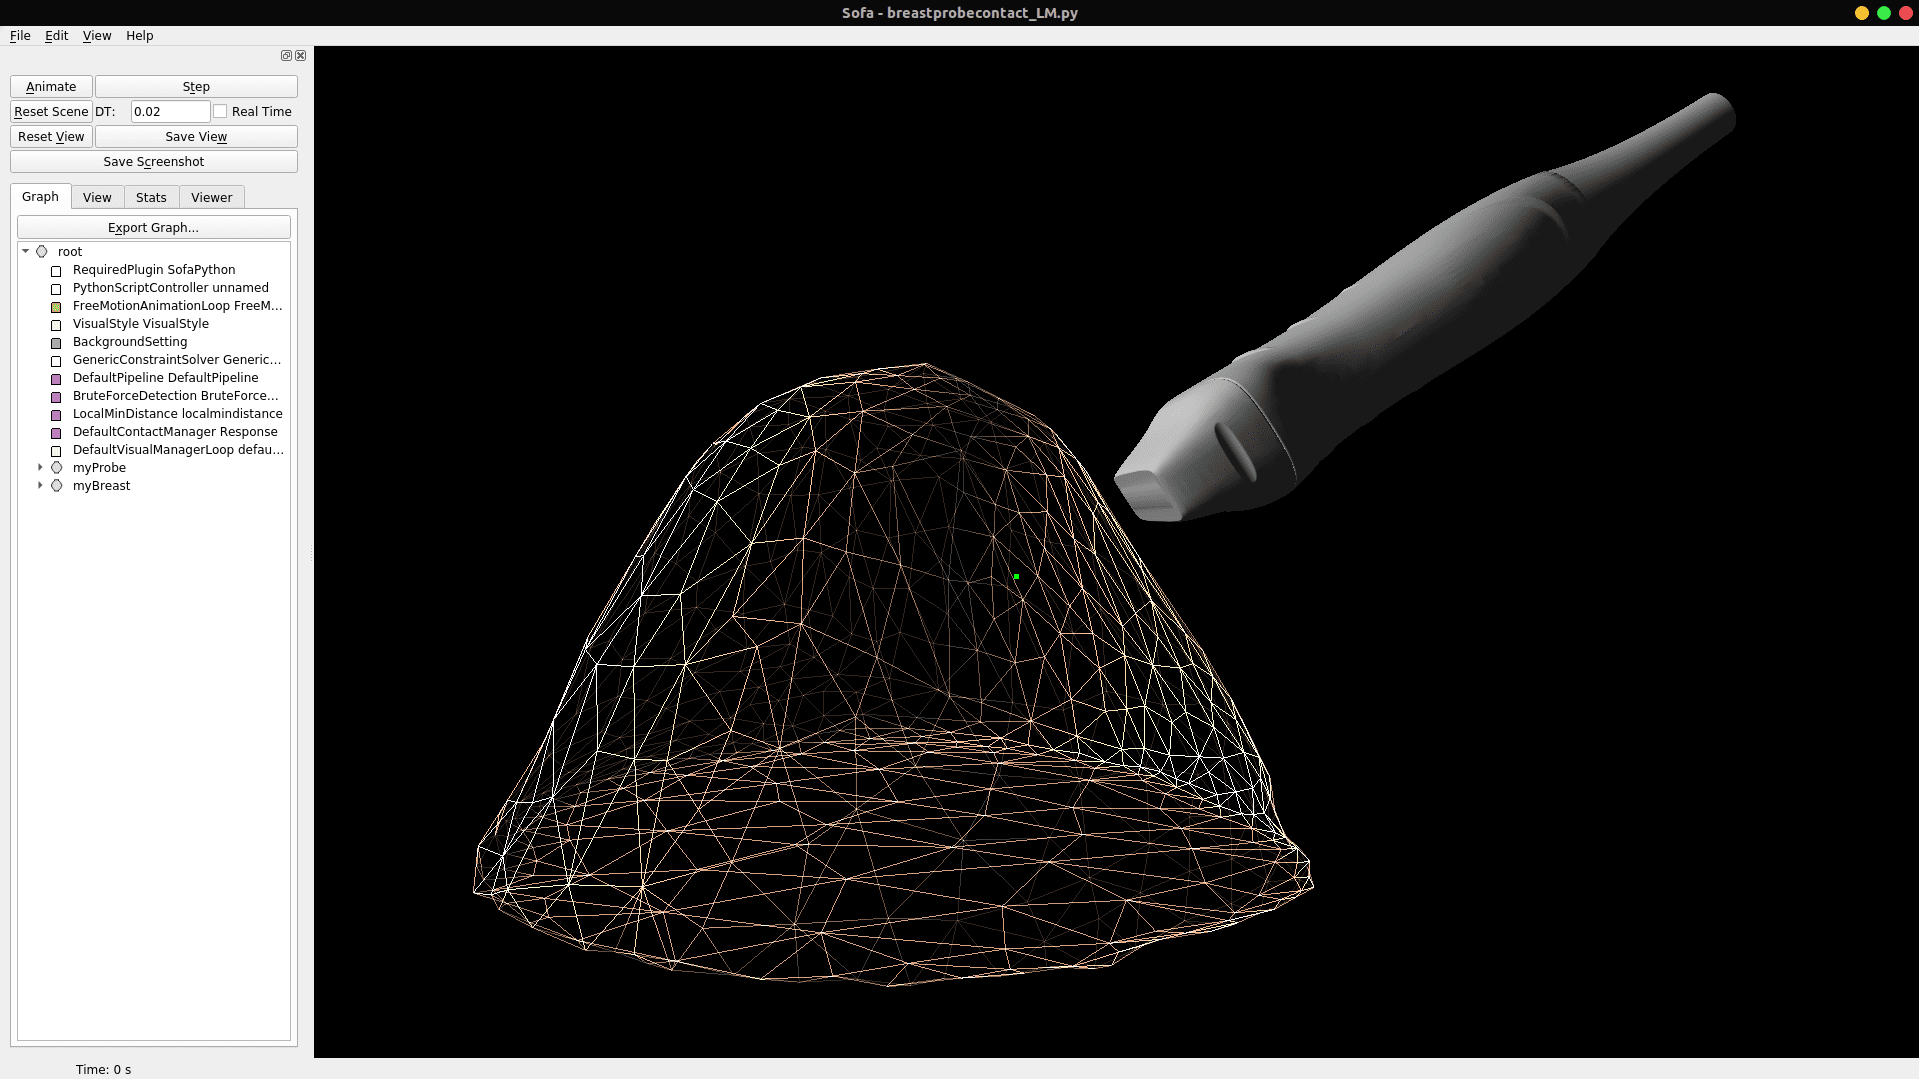
\includegraphics[width=0.4\textwidth]{../images/future-work-sofa1.png}
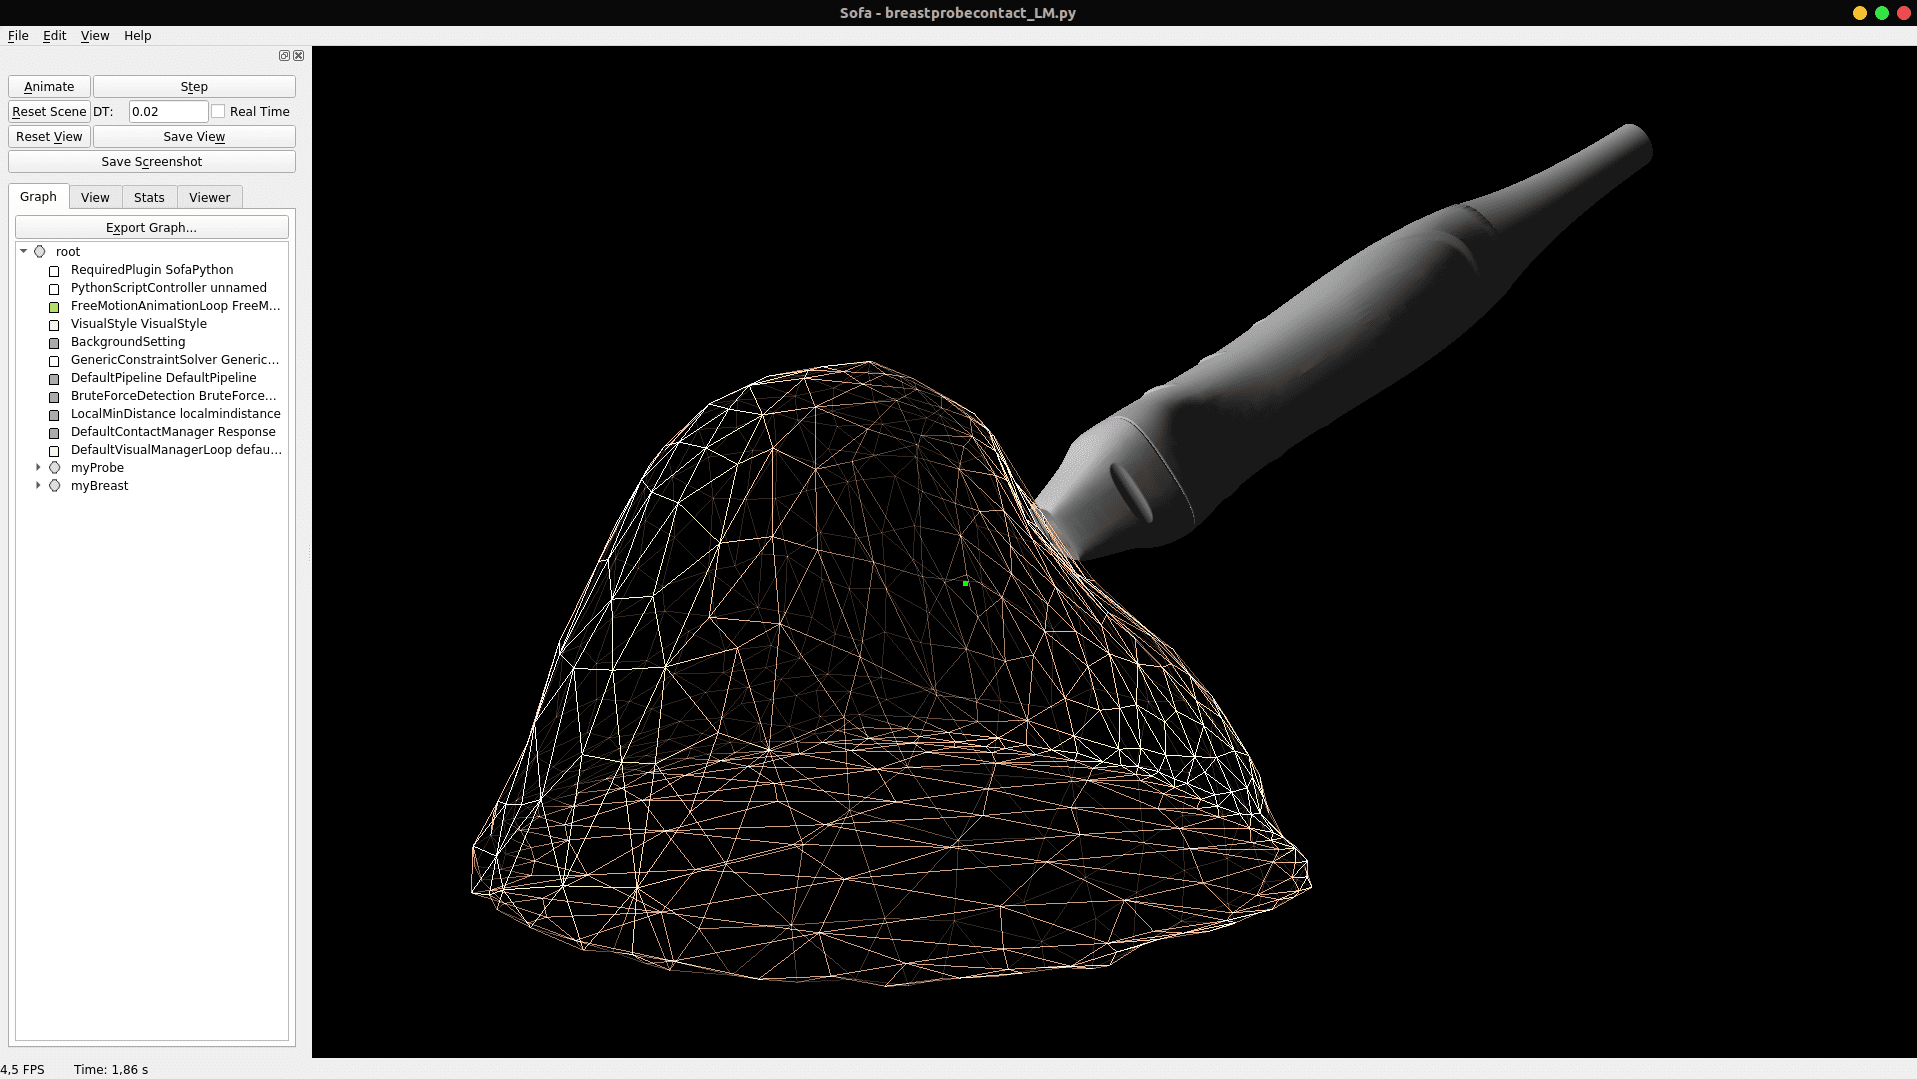
\includegraphics[width=0.4\textwidth]{../images/future-work-sofa2.png}\\
\caption{Soft tissue interaction, deformable objects simulation with the SOFA Framework}
\end{figure}
\end{center}
\end{frame}

\begin{frame}
\frametitle{Code \& Documentation}

\begin{center}
\begin{figure}[!htb]
\centering
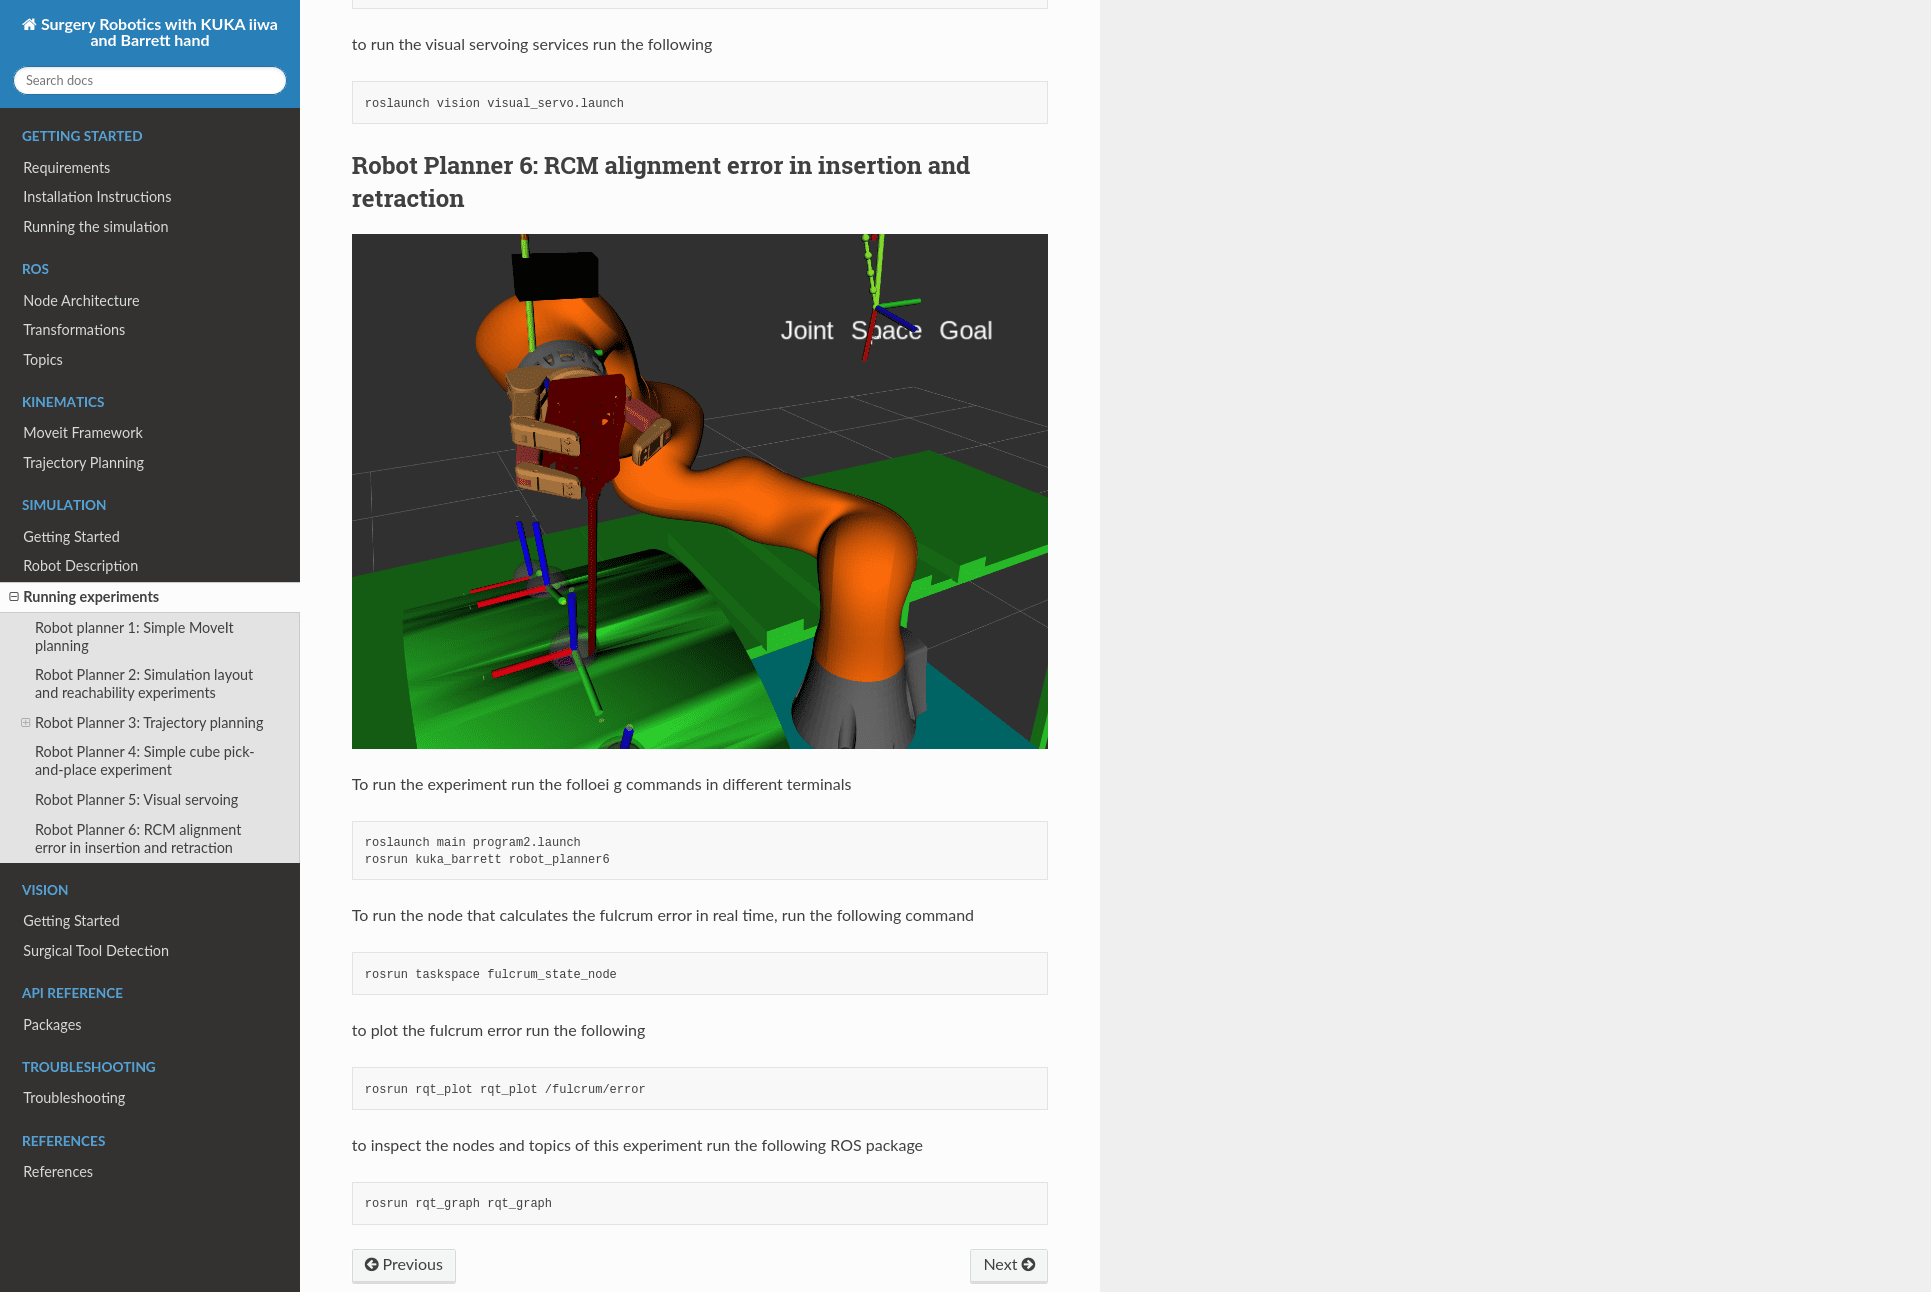
\includegraphics[width=0.5\textwidth]{../images/documentation.png}
\end{figure}
\end{center}

\begin{itemize}
\item Git repository: \textbf{\url{https://github.com/karadalex/surgery_robotics_kuka_barrett}}
\item Documentation: \textbf{\url{https://karadalex.github.io/surgery_robotics_kuka_barrett/}}
\end{itemize}

\end{frame}


\begin{frame}
\frametitle{Questions}

\begin{center}
\begingroup
    \fontsize{14pt}{20pt}\selectfont
    \textbf{Questions?}\\
\endgroup

\vfill
Thank you,\\

\vfill
\begin{center}
\begin{figure}[!htb]
\centering

\includegraphics[width=0.3\textwidth]{../images/contact-info.png}
\end{figure}
\end{center}
\end{center}
\end{frame}